\section{Result}

\section{Results}

\subsection{Measurement for natural angular frequency}
We calculate the angular frequency from Table~\ref{data_omega} by the formula
\[
\omega_0=\frac{2\pi}{T}.
\]
\begin{table}[H] 
\centering
\begin{tabular}{|c|c|}
\hline
& $10T[s] \pm 0.001[s]$\\\hline
1 & 15.790  \\\hline
2 & 15.801  \\\hline
3 & 15.778  \\\hline
4 & 15.800  \\\hline
\end{tabular}
\caption{Measurement of ten periods for the natural frequency}
\label{data_omega}
\end{table}

Hence the average value of $10T$ should be calculated as

\[
\overline{10T}=\frac{1}{4}\sum_{i=1}^{4}(10T)_i=15.79225 \pm 0.0107 \ s, \quad
u_{10T,r}=0.07\%. 
\]

The value of $\omega_0$ is

\[
\overline{\omega_0}=\frac{20\pi}{10T}=\frac{20\times3.1416}{15.79225}= 3.9787
\pm 0.006 \  rad/s,\quad u_{\omega_0,r}=0.15\%. 
\]

\subsection{Measurement for damping coefficient}

The damping coefficient can be calculated by the following formula.

\[
\beta=\frac{1}{5T}\ln\frac{\theta_i}{\theta_{i+5}}.
\]


In the experiment, we choose Damping Selection 2.

\begin{table}[H] 
\centering

\begin{tabular}{|c|c|c|c|c|}
\hline

\multicolumn{2}{|c}{Amplitude[$\degree$]$\pm$1[$\degree$]} & 
\multicolumn{2}{|c|}{Amplitude[$\degree$]$\pm$1[$\degree$]} &
$\ln(\theta_i/\theta_{i+5})$\\\hline

$\theta_0$ & 149 & $\theta_5$ & 95 & 0.4501 \\\hline
$\theta_1$ & 136 & $\theta_6$ & 86 & 0.4583 \\\hline
$\theta_2$ & 124 & $\theta_7$ & 79 & 0.4508 \\\hline
$\theta_3$ & 114 & $\theta_8$ & 72 & 0.4595 \\\hline
$\theta_4$ & 103 & $\theta_9$ & 65 & 0.4603 \\\hline
\multicolumn{4}{|c|}{The average value of $\ln(\theta_i/\theta_{i+5})$}
    & 0.4558 \\\hline 
\end{tabular}

\caption{Measurement of the damping coefficient for Damping Selection 2}
\label{data_damping}
\end{table}

The experimental value of $\ln(\theta_i/\theta_{i+5})$ is shown below

\[
\ln(\theta_i/\theta_{i+5})= 0.4558 \pm 0.0050 , \quad u_r=1.09\%
\]

Here, $T= 15.79225 /10= 1.5792 \pm 0.0001s$. Then we can easily obtain $\beta$
as well, 

\[
\beta=\frac{1}{5\times1.5792}\times0.4558=  0.0577 \pm 0.003s^{-1}, \quad
u_{\beta,r}=5.2\% 
\]

\subsection{Measurement for $\theta_{st}$ vs. $\omega$ and $\varphi$ vs. 
  $\omega$} 

To study the relation between $\varphi$ and $\omega/\omega_0$, 

first we get the raw data of 10T, $\phi$ and $\theta$,
we then process the raw data and list them in Table~\ref{data_phi2} and
Table~\ref{data_phi3}. 


\begin{table}[H]
\centering
\begin{tabular}{|c|c|c|c|}
\hline
& $10T [s] \pm 0.001 [s]$ &  $\varphi  [\degree]  \pm 1 [\degree]$ & $ \theta [\degree] \pm 1 [\degree]$ \\ \hline

1  & 15.098 & -162  &  38   \\ \hline
2  & 15.123 & -163  &  39   \\ \hline
3  & 15.542 & -143  &  87   \\ \hline
4  & 15.672 & -118  &  130  \\ \hline
5  & 15.707 & -109  &  138  \\ \hline
6  & 15.724 & -103  &  141  \\ \hline
7  & 15.736 & -100  &  143  \\ \hline
8  & 15.755 & -94   &  145  \\ \hline
9  & 15.763 & -92   &  146  \\ \hline
10 & 15.774 & -89   &  144  \\ \hline
11 & 15.788 & -86   &  144  \\ \hline
12 & 15.797 & -84   &  144  \\ \hline
13 & 15.810 & -82   &  144  \\ \hline
14 & 15.820 & -79   &  142  \\ \hline
15 & 15.841 & -75   &  140  \\ \hline
16 & 15.907 & -64   &  130  \\ \hline
17 & 15.946 & -57   &  124  \\ \hline
18 & 16.050 & -46   &  105  \\ \hline
19 & 16.131 & -40   &  92   \\ \hline
20 & 16.237 & -33   &  78   \\ \hline
21 & 16.472 & -22   &  54   \\ \hline
22 & 16.603 & -18   &  46   \\ \hline
\end{tabular}    
\caption{$\theta$ vs. $10T$ and $\varphi$ vs. $10T$ raw data for Damping selection 2}
\end{table}

\begin{table}[H]
\centering
\begin{tabular}{|c|c|c|c|}
\hline
& $10T [s] \pm 0.001 [s]$ &  $\varphi  [\degree]  \pm 1 [\degree]$ & $ \theta [\degree] \pm 1 [\degree]$ \\ \hline

1  & 15.057   & -163 &  35   \\ \hline
2  & 15.302   & -155 &  50   \\ \hline
3  & 15.526   & -142 &  79   \\ \hline
4  & 15.657   & -123 &  108  \\ \hline
5  & 15.708   & -111 &  120  \\ \hline
6  & 15.745   & -104 &  125  \\ \hline
7  & 15.760   & -97  &  127  \\ \hline
8  & 15.794   & -93  &  128  \\ \hline
9  & 15.789   & -92  &  128  \\ \hline
10 & 15.803   & -89  &  128  \\ \hline
11 & 15.814   & -86  &  128  \\ \hline
12 & 15.830   & -83  &  128  \\ \hline
13 & 15.849   & -80  &  126  \\ \hline
14 & 15.883   & -74  &  124  \\ \hline
15 & 15.903   & -69  &  120  \\ \hline
16 & 15.933   & -62  &  114  \\ \hline
17 & 16.013   & -55  &  106  \\ \hline
18 & 16.102   & -47  &  93   \\ \hline
19 & 16.168   & -41  &  83   \\ \hline
20 & 16.290   & -33  &  70   \\ \hline
21 & 16.452   & -25  &  55   \\ \hline
22 & 16.585   & -18  &  46   \\ \hline
\end{tabular}    
\caption{$\theta$ vs. $10T$ and $\varphi$ vs. $10T$ raw data for Damping selection 3}
\end{table}


Then We know that $ \omega / \omega_0 = T_0 / T $,
thus we can have the following processed data.


\begin{table}[H]
\centering
\begin{tabular}{|c|c|c|}
\hline
& $\omega/\omega_0$ &  $\varphi \pm 1 [\degree] $ \\ \hline
1  & 1.0460  & -162  \\ \hline
2  & 1.0443  & -163  \\ \hline
3  & 1.0161  & -143  \\ \hline
4  & 1.0077  & -118  \\ \hline
5  & 1.0054  & -109  \\ \hline
6  & 1.0043  & -103  \\ \hline
7  & 1.0036  & -100  \\ \hline
8  & 1.0024  & -94   \\ \hline
9  & 1.0019  & -92   \\ \hline
10 & 1.0012  & -89   \\ \hline
11 & 1.0003  & -86   \\ \hline
12 & 0.9997  & -84   \\ \hline
13 & 0.9989  & -82   \\ \hline
14 & 0.9982  & -79   \\ \hline
15 & 0.9969  & -75   \\ \hline
16 & 0.9928  & -64   \\ \hline
17 & 0.9904  & -57   \\ \hline
18 & 0.9839  & -46   \\ \hline
19 & 0.9790  & -40   \\ \hline
20 & 0.9726  & -33   \\ \hline
21 & 0.9587  & -22   \\ \hline
22 & 0.9512  & -18   \\ \hline
\end{tabular}    
\caption{$\varphi$ vs. $\omega/\omega_0$, Damping selection 2}\label{data_phi2}
\end{table}

\begin{table}[H]
\centering
\begin{tabular}{|c|c|c|}
\hline
& $\omega/\omega_0$ &  $\varphi \pm 1 [\degree] $ \\ \hline
1  & 1.0488   & -163 \\ \hline
2  & 1.0320   & -155 \\ \hline
3  & 1.0171   & -142 \\ \hline
4  & 1.0086   & -123 \\ \hline
5  & 1.0054   & -111 \\ \hline
6  & 1.0030   & -104 \\ \hline
7  & 1.0020   &  -97 \\ \hline
8  & 0.9999   &  -93 \\ \hline
9  & 1.0002   &  -92 \\ \hline
10 & 0.9993   &  -89 \\ \hline
11 & 0.9986   &  -86 \\ \hline
12 & 0.9976   &  -83 \\ \hline
13 & 0.9964   &  -80 \\ \hline
14 & 0.9943   &  -74 \\ \hline
15 & 0.9930   &  -69 \\ \hline
16 & 0.9912   &  -62 \\ \hline
17 & 0.9862   &  -55 \\ \hline
18 & 0.9808   &  -47 \\ \hline
19 & 0.9768   &  -41 \\ \hline
20 & 0.9694   &  -33 \\ \hline
21 & 0.9599   &  -25 \\ \hline
22 & 0.9522   &  -18 \\ \hline
\end{tabular}    
\caption{$\varphi$ vs. $\omega/\omega_0$, Damping selection 3}\label{data_phi3}
\end{table}




\begin{figure}[H]
\centering
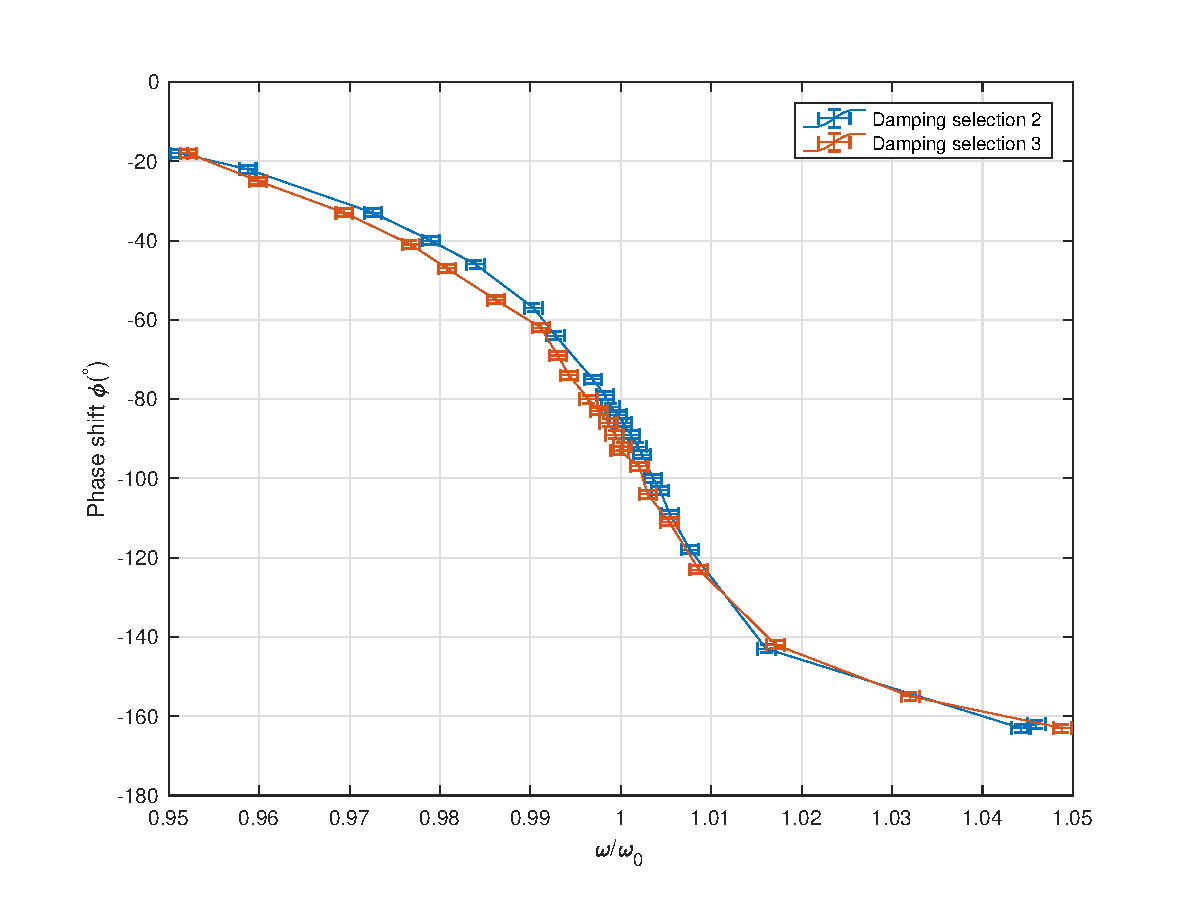
\includegraphics[width=1\textwidth]{matlab/p1}
\caption{Phase shift $\varphi$ vs. $\omega/\omega_0$}\label{phi}
\end{figure}


To study the relation between $\theta_{st}$ and $\omega/\omega_0$, we process the raw data and list them in Table \ref{data_theta2} and \ref{data_theta3}.


% TODO:

\begin{figure}[H]
\centering
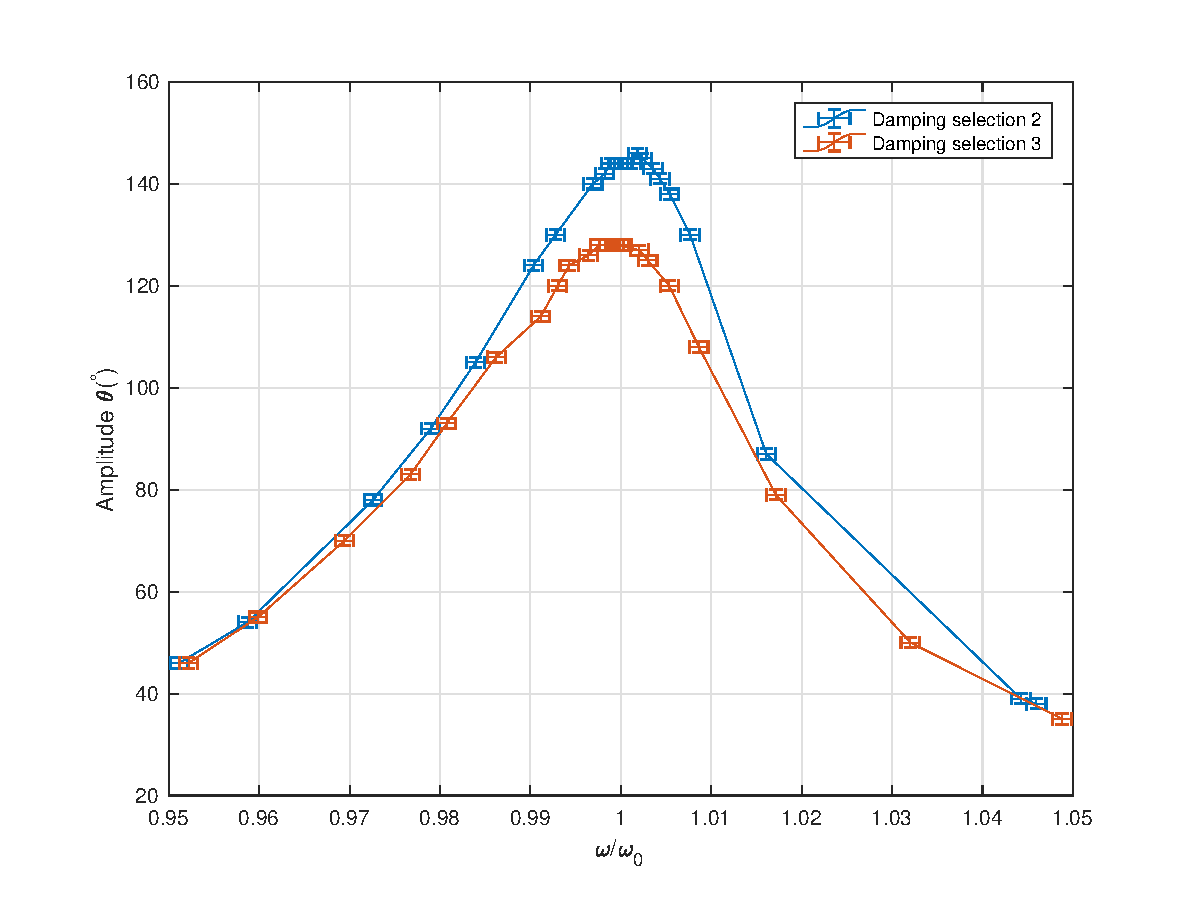
\includegraphics[width=1\textwidth]{matlab/p2}
\caption{Amplitude $\theta_{st}$ vs. $\omega/\omega_0$}\label{theta}
\end{figure}






\begin{table}[H]
\centering
\begin{tabular}{|c|c|c|c|c|}
\hline
                No. & $\omega/\omega_0[\ ]$ & $u_{\omega/\omega_0}[\ ]$ & $\theta_{st}[\degree]$ & $u_{\theta_{st}}[\degree]$\\\hline
                1 & 1.0416 & 0.0010 & 42 & 1\\\hline
                2 & 1.0296 & 0.0010 & 56 & 1\\\hline
                3 & 1.0187 & 0.0010 & 78 & 1\\\hline
                4 & 1.0110 & 0.0010 & 107 & 1\\\hline
                5 & 1.0075 & 0.0010 & 123 & 1\\\hline
                6 & 1.0050 & 0.0010 & 132 & 1\\\hline
                7 & 1.0032 & 0.0010 & 138 & 1\\\hline
                8 & 1.0018 & 0.0010 & 140 & 1\\\hline
                9 & 1.0011 & 0.0010 & 140 & 1\\\hline
                10 & 1.0006 & 0.0010 & 141 & 1\\\hline
                11 & 0.9998 & 0.0010 & 140 & 1\\\hline
                12 & 0.9980 & 0.0010 & 140 & 1\\\hline
                13 & 0.9965 & 0.0010 & 138 & 1\\\hline
                14 & 0.9943 & 0.0010 & 134 & 1\\\hline
                15 & 0.9915 & 0.0010 & 126 & 1\\\hline
                16 & 0.9892 & 0.0010 & 121 & 1\\\hline
                17 & 0.9870 & 0.0010 & 116 & 1\\\hline
                18 & 0.9860 & 0.0010 & 112 & 1\\\hline
                19 & 0.9843 & 0.0010 & 106 & 1\\\hline
                20 & 0.9812 & 0.0010 & 98 & 1\\\hline
                21 & 0.9772 & 0.0010 & 88 & 1\\\hline
                22 & 0.9712 & 0.0010 & 76 & 1\\\hline
                23 & 0.9640 & 0.0010 & 64 & 1\\\hline
            \end{tabular}
            \caption{$\theta_{st}$ and $\omega/\omega_0$, Damping selection 2}\label{data_theta2}
        \end{table}

        \begin{table}[H]
        \centering
            \begin{tabular}{|c|c|c|c|c|}
                \hline
                No. & $\omega/\omega_0[\ ]$ & $u_{\omega/\omega_0}[\ ]$ & $\theta_{st}[\degree]$ & $u_{\theta_{st}}[\degree]$\\\hline
                1 & 0.9624 & 0.0010 & 60 & 1\\\hline
                2 & 0.9669 & 0.0010 & 67 & 1\\\hline
                3 & 0.9715 & 0.0010 & 74 & 1\\\hline
                4 & 0.9771 & 0.0010 & 86 & 1\\\hline
                5 & 0.9818 & 0.0010 & 96 & 1\\\hline
                6 & 0.9868 & 0.0010 & 108 & 1\\\hline
                7 & 0.9925 & 0.0010 & 120 & 1\\\hline
                8 & 0.9954 & 0.0010 & 124 & 1\\\hline
                9 & 0.9971 & 0.0010 & 126 & 1\\\hline
                10 & 0.9976 & 0.0010 & 128 & 1\\\hline
                11 & 1.0004 & 0.0010 & 128 & 1\\\hline
                12 & 1.0022 & 0.0010 & 126 & 1\\\hline
                13 & 1.0039 & 0.0010 & 124 & 1\\\hline
                14 & 1.0056 & 0.0010 & 120 & 1\\\hline
                15 & 1.0068 & 0.0010 & 115 & 1\\\hline
                16 & 1.0083 & 0.0010 & 110 & 1\\\hline
                17 & 1.0107 & 0.0010 & 100 & 1\\\hline
                18 & 1.0132 & 0.0010 & 90 & 1\\\hline
                19 & 1.0158 & 0.0010 & 82 & 1\\\hline
                20 & 1.0191 & 0.0010 & 74 & 1\\\hline
                21 & 1.0221 & 0.0010 & 66 & 1\\\hline
                22 & 1.0290 & 0.0010 & 56 & 1\\\hline
                23 & 1.0367 & 0.0010 & 46 & 1\\\hline
            \end{tabular}
            \caption{$\theta_{st}$ and $\omega/\omega_0$, Damping selection 3}\label{data_theta3}
        \end{table}
